\chapter{Función exponencial}\label{Apendice_A}
En este apéndice, se lleva a cabo una comparación  de los factores $\rho$ en la función exponencial, examinando cómo estos parámetros ejercen una influencia en la forma de la función. Esta comparación se presenta de manera concisa pero exhaustiva, explorando las variaciones en el comportamiento de la función exponencial en función de los valores de $\rho$.

\section{Comparación}
Es relevante observar que en la ecuación (\ref{eq 2}), la desviación de una función exponencial con parámetro $\rho$ se evalúa 
$D(t) = \exp( - \rho t)(1 + \varepsilon(t)).$ 
Se comparará exclusivamente la función exponencial $\exp(-\rho t)$.

\begin{figure}[!h]
\begin{center}
\vspace{-0.4cm}
\includegraphics[width=0.495\textwidth]{10_ApendiceA/graficos/graf.eps}
\vspace{-0.4cm} 
\caption{Gráfico de $e^{- \rho t}$ para distintos valores de $\rho$.}
\vspace{-0.0cm}
\label{fig_comparación}
\end{center}
\end{figure}
